\documentclass[11pt, a4paper, english]{NTNUoving}
\usepackage[utf8]{inputenc}
\usepackage[T1]{fontenc}
\usepackage{float}
\usepackage{enumitem}
\usepackage{csquotes}
\usepackage{listings}
\usepackage{color}
\usepackage{biblatex}
\usepackage{hyperref}
\usepackage{multirow}
\usepackage{hyperref}
\usepackage{pdfpages}

\addbibresource{references.bib}


\ovingnr{2}    % Nummer på innlevering
\semester{Spring 2021}
\fag{Methods in Artificial Inteligence \\ TDT4171}
\institutt{Department for Computer Science}

\begin{document}
\begin{oppgave}

\begin{punkt}

The Bayesian network for this problem is shown in figure Figure \ref{fig:1}.

\begin{figure}[h]
    \centering
    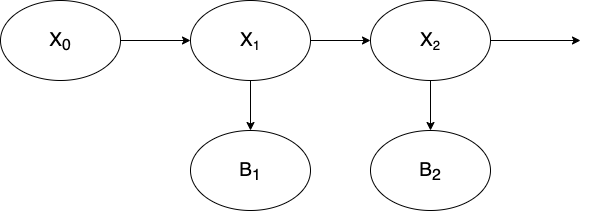
\includegraphics[width=0.5\textwidth]{BN1.png}
    \caption{Bayesian network for the problem.}
    \label{fig:1}
\end{figure}

Here $X_t$ is the state distribution on time $t$ and $B_t$ is the evidence distribution at time $t$.

The probability distributions are be given by tables \ref{tab:1}, \ref{tab:2} and \ref{tab:3}.

\begin{table}[H]
    \centering
    \begin{tabular}{|c|c|c|}
        \hline
       & \multicolumn{2}{|c|}{$P(X_t)$} \\ [0.5ex]
        \hline
        $X_{t-1}$ & $t$ & $f$ \\
        \hline
        $t$ & 0.8 & 0.2 \\ [1.0ex]
        $f$ & 0.3 & 0.7\\ [1.0ex]
        \hline
\end{tabular}
    \caption{Probability distribution for $P(X_t | X_{t-1})$.}
    \label{tab:1}
\end{table}

\begin{table}[H]
    \centering
    \begin{tabular}{|c|c|c|}
        \hline
       & \multicolumn{2}{|c|}{$P(B_t)$} \\ [0.5ex]
        \hline
        $X_t$ & $t$ & $f$ \\
        \hline
        $t$ & 0.75 & 0.25 \\ [1.0ex]
        $f$ & 0.2 & 0.8\\ [1.0ex]
        \hline
\end{tabular}
    \caption{Probability distribution for $P(B_t | X_t)$.}
    \label{tab:2}
\end{table}

\begin{table}[H]
    \centering
    \begin{tabular}{|c|c|}
        \hline
       \multicolumn{2}{|c|}{$P(X_0)$} \\ [0.5ex]
        \hline
        $t$ & $f$ \\
        \hline
        0.5 & 0.5 \\ [1.0ex]
        \hline
\end{tabular}
    \caption{Probability distribution for $P(X_0)$.}
    \label{tab:3}
\end{table}

Formulation as a hidden Markov model:

\begin{align*}
    \textbf{T} = \begin{bmatrix}
        0.8 & 0.2\\
        0.3 & 0.7
    \end{bmatrix} \\
    \textbf{P}(X_0) = \begin{bmatrix}
        0.5\\
        0.5
    \end{bmatrix}
\end{align*}

$\textbf{T}$ is the transition model and
$\textbf{P}(X_0)$ is the initial distribution.

The sensor model $\textbf{O}_t$ depends on the evidence given:
\begin{align*}
    \textbf{e}_t &= BirdsNearby \implies \textbf{O}_t = \begin{bmatrix}
        0.75 & 0\\
        0 & 0.2
    \end{bmatrix} \\
    \textbf{e}_t &= NoBirdsNearby \implies \textbf{O}_t = \begin{bmatrix}
        0.25 & 0\\
        0 & 0.8
    \end{bmatrix}
\end{align*}
\end{punkt}

\begin{punkt}

    This kind of operation is filtering, where we calculate the current belief state given all the evidence to date.
    The results are given in Figure \ref{fig:filtering}. This operation gives us the probability distribution of the current state given all the evidence to date.
    \begin{figure}[H]
        \centering
        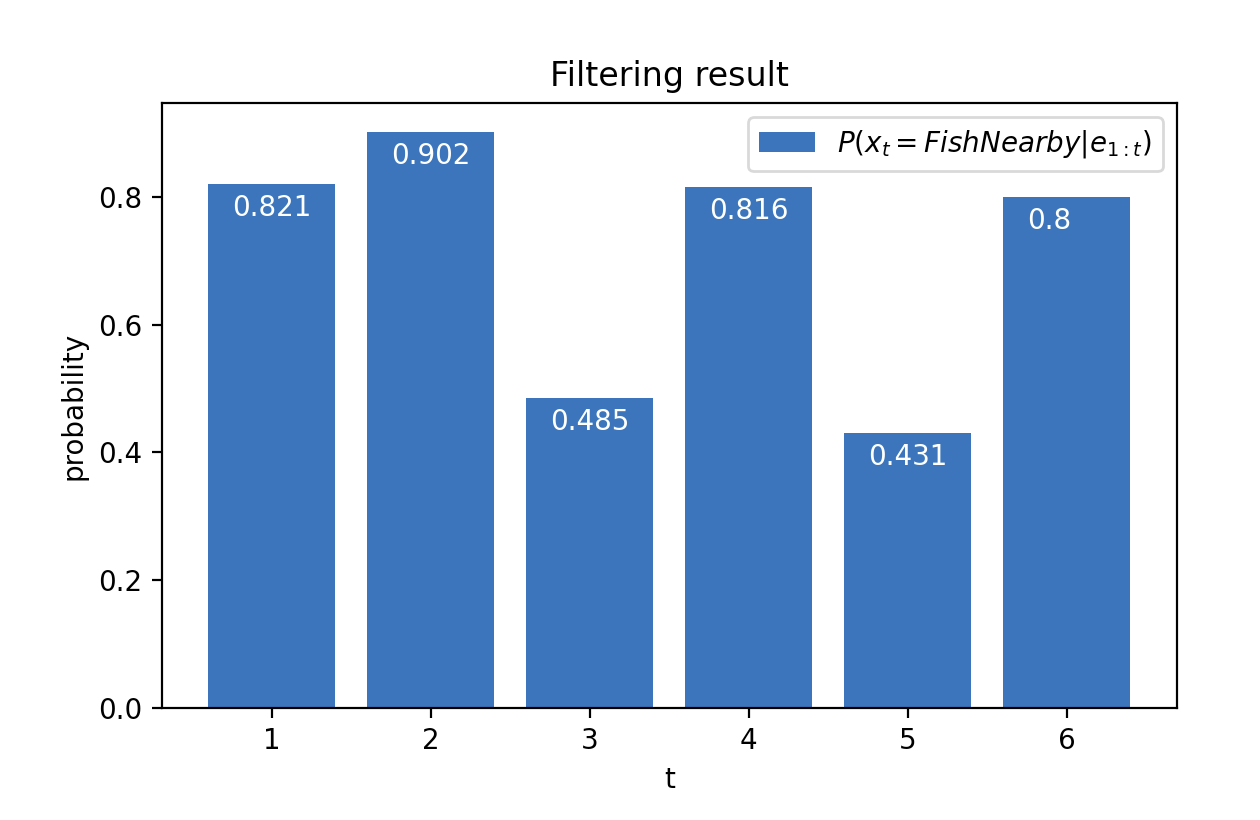
\includegraphics[width=0.5\textwidth]{filtering.png}
        \caption{Filtering for $t = 1,...,6$.}
        \label{fig:filtering}
    \end{figure}

    As we can see the filtering results vary with the evidence, when we observe birds nearby the probability of fish nearby is also high, while when there are no birds nearby
    the probability of fish nearby is lower, which makes sense from the transition and sensor model.

\end{punkt}

\begin{punkt}

    This kind of operation is prediction, where we calculate the distribution of a future state, based on the previous evidence, but no new addition evidence are given.
    This is the same as filtering without adding new evidence. The results are given in Figure \ref{fig:prediction}.
    \begin{figure}[H]
        \centering
        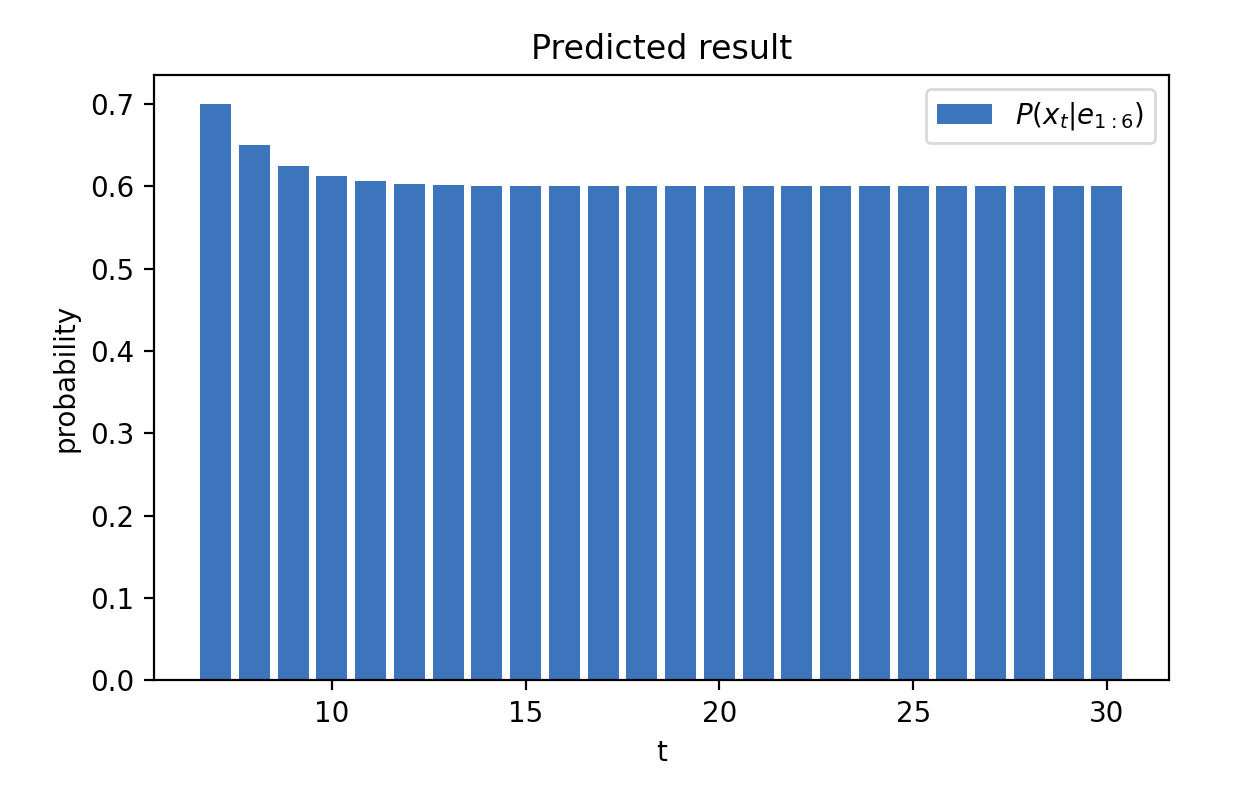
\includegraphics[width=0.5\textwidth]{prediction.png}
        \caption{Prediction for $t = 7,...,30$.}
        \label{fig:prediction}
    \end{figure}
    As we can see, the belief state converges towards $\begin{bmatrix}
        0.6 & 0.4
    \end{bmatrix}^\top$ as $t$ increases. This is because $\begin{bmatrix}
        0.6 & 0.4
    \end{bmatrix}^\top$ is the eigenvector for the eigenvalue $1$ in the matrix $T^\top$. This will be explained further in Task 2b.
\end{punkt}

\begin{punkt}
    This kind of operation is smoothing, where we calculate the distribution of a past state, given all the evidence up to the present.
    The results are given in Figure \ref{fig:smoothing}.

    \begin{figure}[H]
        \centering
        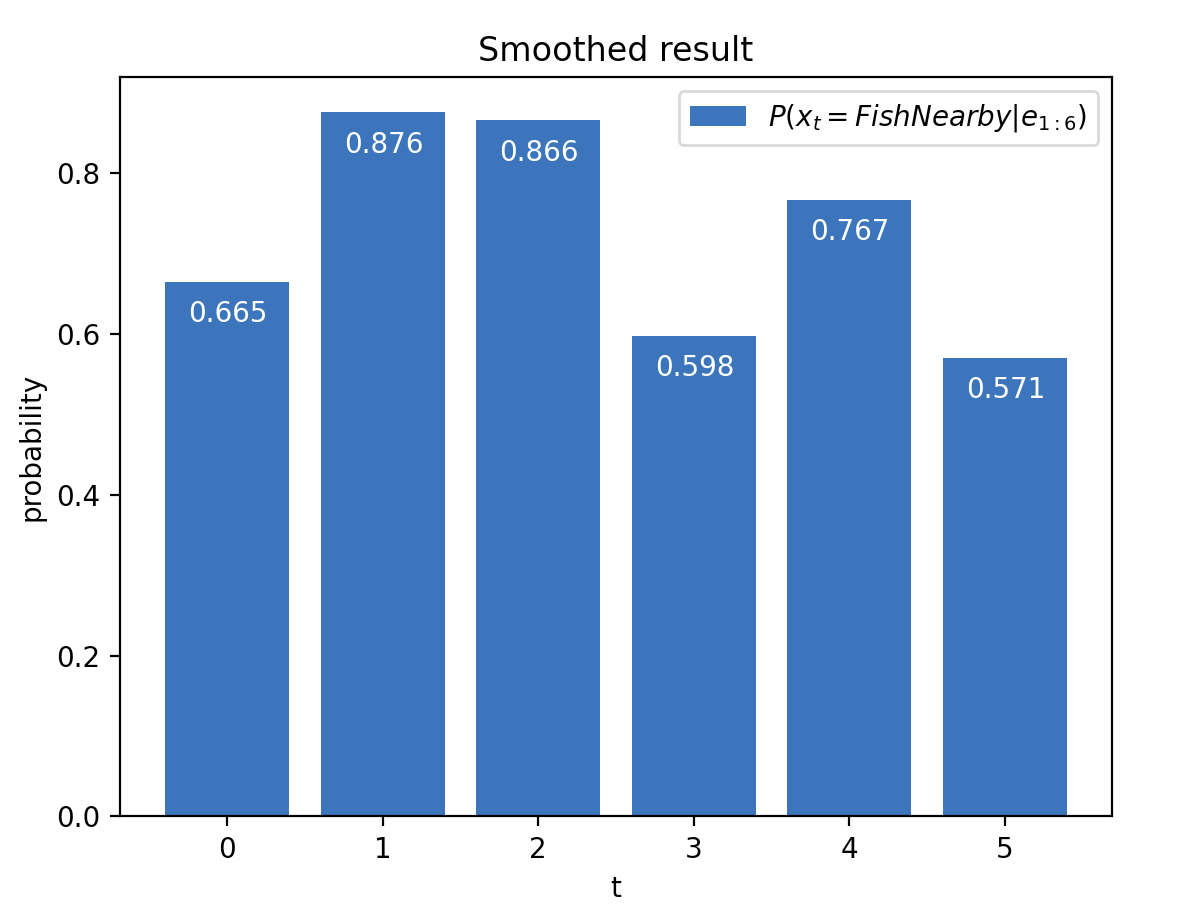
\includegraphics[width=0.5\textwidth]{smoothing.png}
        \caption{Smoothing for $t = 0,...,5$.}
        \label{fig:smoothing}
    \end{figure}

    As we can see the smoothed results gives a higher probability of fish nearby when there are no birds nearby than filtering.
    For example on day 3 the smoothed result is 0.598 while the filtered is 0.485, this is because the birds nearby on day 4 makes it more
    likely to be fish nearby on day 3 since fish nearby tends to persist.
\end{punkt}

\begin{punkt}
    This kind of operation is most likely sequence, where we calculate the most like sequence of states given all the evidence up to the present.
    The results where the sequence given in Figure \ref{fig:viterbi}.

    \begin{figure}[H]
        \centering
        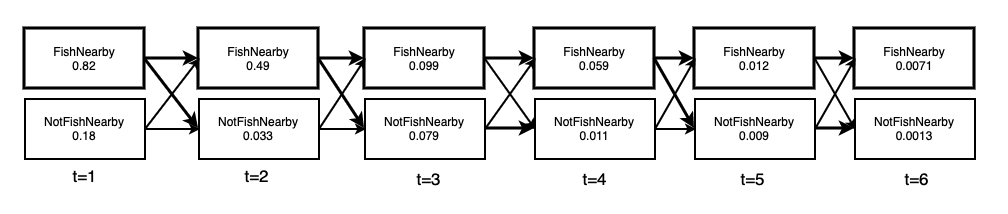
\includegraphics[width=1.0\textwidth]{viterbi.png}
        \caption{Viterbi sequence for $t = 1,...,6$.}
        \label{fig:viterbi}
    \end{figure}

    We see that the most likely sequence for $X_6 = FishNearby$ is the sequence of
    $0, 0, 0, 0, 0$ for $t=1,...,5$ respectively, while the most likely sequence for
    $X_6=NoFishNearby$ is the sequence $0, 0, 0, 0, 1$. (Here $0=FishNearby,\;1=NoFishNearby$.)
    We see that the algorithm choose $X_6 = FishNearby$ as this has a higher probability.
\end{punkt}

\end{oppgave}
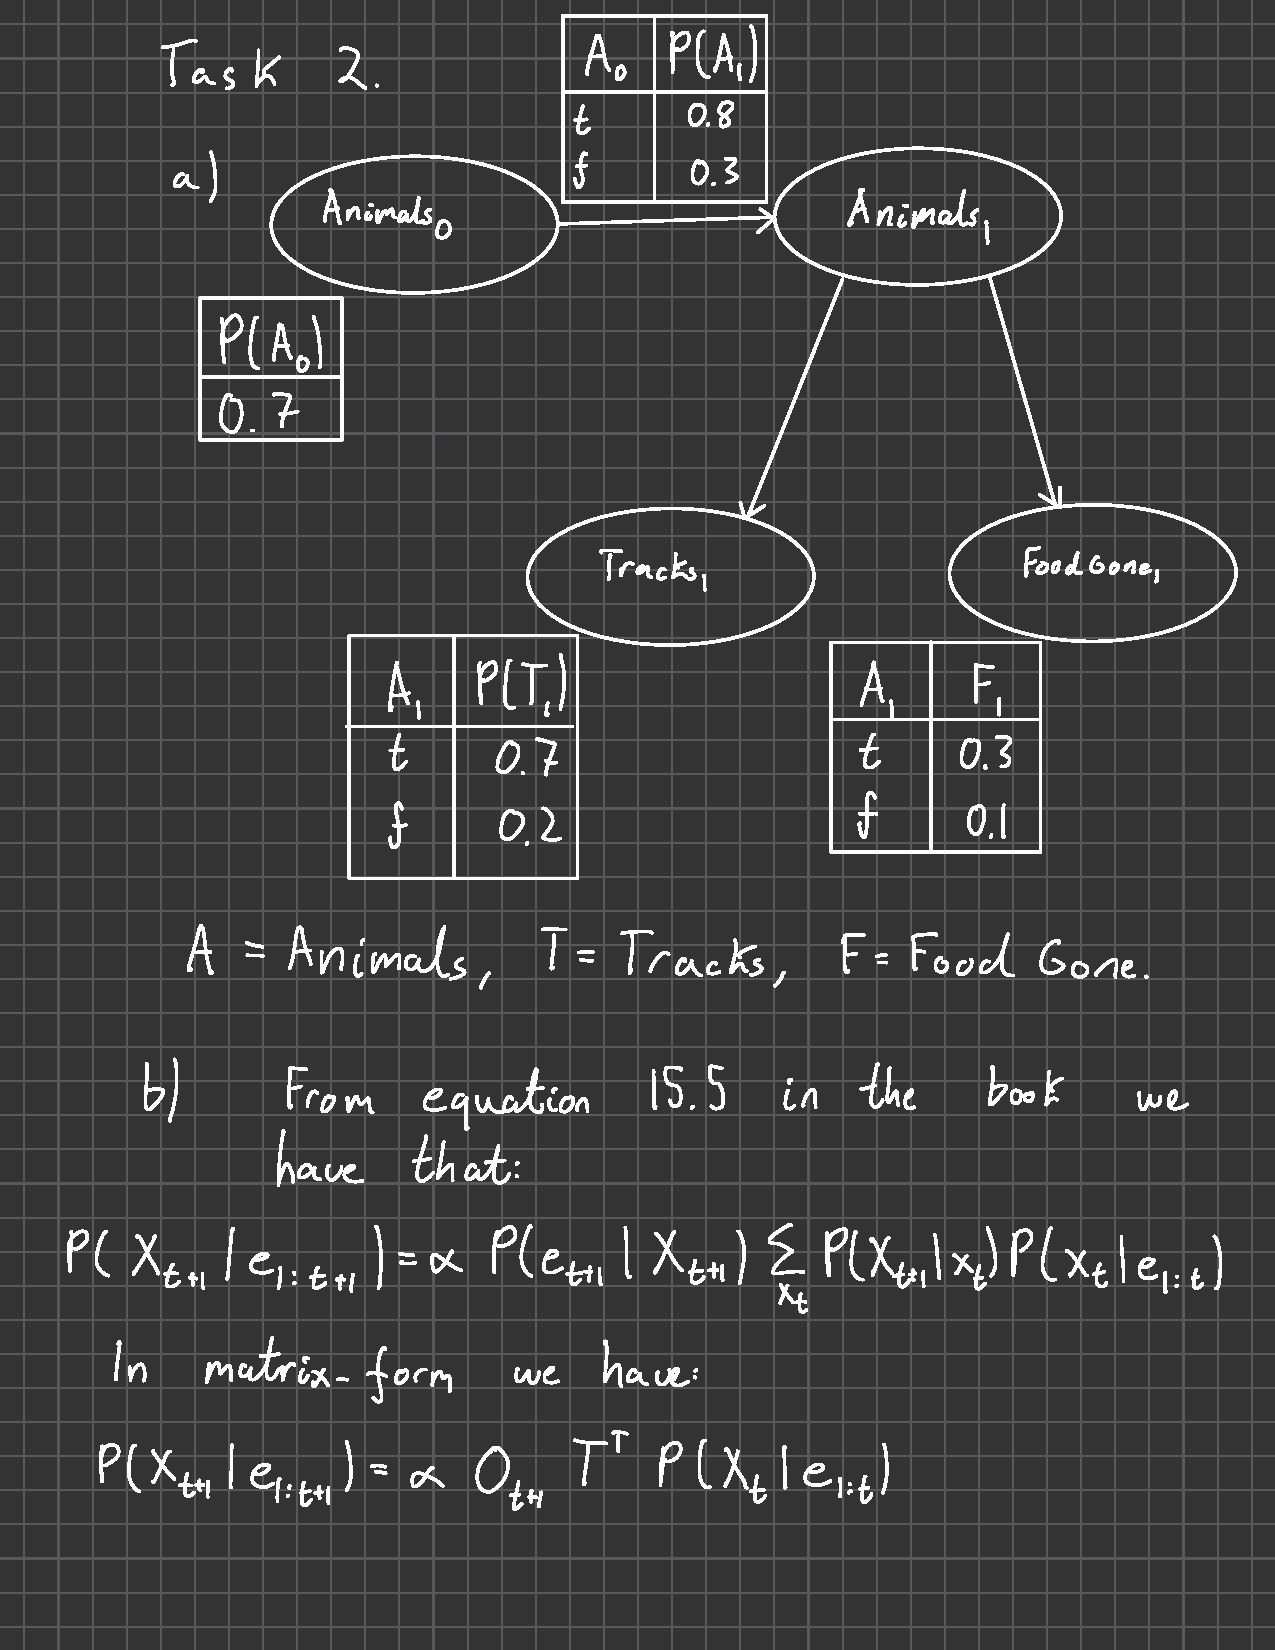
\includepdf[pages=-]{task2.pdf}
\end{document}
